\documentclass[a4paper,12pt]{article}


\usepackage{amsmath}
\usepackage{authblk}
\usepackage{booktabs}
\usepackage[margin=1in]{geometry}
\usepackage{mathtools}
\usepackage{dsfont}
\usepackage{bm}
\usepackage{mdframed}
\usepackage{amsthm}
\usepackage{xfrac}
\usepackage{tikz}
\usetikzlibrary{arrows}

\newcommand{\p}[1]{\mathds{P}\left\{#1 \right\}}
\newcommand{\pp}[1]{\mathds{P}_{\phi} \left\{#1 \right\}}
\newcommand{\pth}[1]{\mathds{P}_{\vartheta} \left\{#1 \right\}}
\newcommand{\pph}[1]{\mathds{P}_{\phi_h} \left\{#1 \right\}}
\newcommand{\ppt}[1]{\mathds{P}_{\phi_t} \left\{#1 \right\}}
\newcommand{\e}[1]{\mathds{E}[#1]}

\newcommand{\fca}{\phi_{\text{case}}}
\newcommand{\fco}{\phi_{\text{control}}}

%opening
\title{Non-nested models?}
\author{Louis Dijkstra}

\begin{document}

\maketitle

Suppose we have the obtained a likelihood function for the parameter $\vartheta = (\phi, \psi)$ given the data $x$: 
$$
  \mathcal{L}(\vartheta ; x) = \mathds{P}_{\vartheta} \{x\}. 
$$
The parameter $\vartheta$ lies in the parameter space 
$$
  \Theta = \{(\phi, \psi) : \phi \in \{0, \sfrac{1}{2}, 1\}, \psi \in [0,1]\}.
$$
We want to determine whether the parameter $\vartheta$ lies within the subspace
$$
  \vartheta \in \Theta_0 = \{0,0\} \cup \{(\phi, \psi) : \phi \in \{\sfrac{1}{2}, 1\}, \psi \in [0,1]\} 
$$
or 
$$
  \vartheta \in \Theta_1 = \{(\phi, \psi) : \phi = 0, \psi \in (0,1]\}, 
$$
(where the former responds to the case where there is no somatic mutation, i.e., healty cells do not differ from tumor cells in this region of the \textsc{dna}, and the latter reflects the situation where a somatic mutation occured, i.e., tumor cells differ from healthy cells). See Figure 1 for a graphical depiction. I feel that the appropriate null- and alternative hypothesis are
$$
  H_0 : \vartheta \in \Theta_0 \text{ (no somatic mutation)} \quad \text{vs.} \quad H_1 : \vartheta \in \Theta_1 \text{ (somatic mutation)}. 
$$
My question is: is this a non-nested case? Or would the classical likelihood ratio test do? 




\begin{figure}
  \centering
 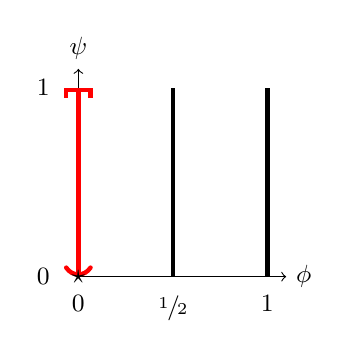
\begin{tikzpicture}[scale = 1.2]
  \draw[->] (0,0) -- (0,2.2) node [above] {\small $\psi$} ; 
  \draw[->] (0,0) -- (2.2,0)  node [right] {\small $\phi$} ; 
  
  %\draw[ultra thick] node[below] {\small $0$} (0,0) -- (0,2) ;
  \draw[ultra thick] (1,0) -- (1,2) ; 
  \draw[ultra thick] (2,0) -- (2,2) ; 
  
  \draw node[below] at (0,-0.1) {\small $0$} ; 
  \draw node[below] at (1,-0.1) {\small $\sfrac{1}{2}$} ; 
  \draw node[below] at (2,-0.1) {\small $1$} ; 
  \draw node[left] at (-0.2,0) {\small $0$} ; 
  \draw node[left] at (-0.2,2) {\small $1$} ; 
  \draw[[-), ultra thick, red] (0,2) -- (0,0);
  \draw node at (0,0) {$\star$} ; 
 \end{tikzpicture}
 \caption{The parameter space $\Theta$. The red interval $(0,1]$ at $\phi = 0$ is $\Theta_1$ and denotes the cases where a somatic mutation occured. The parameters related to the situation where no mutation occured are depicted with black, including the origin $(0,0)$ which is for clarity shown here with a $\star$. }
\end{figure}

\end{document}